\textsf{
Mange af de metoder, vi bruger til at udregne, det gyldne snits position
eller størrelsen af en margin, udregnes med brøker. Hvorimod et billede
opbygges af pixels. Dette gør, at vi bliver nødt til at tage
approksimationer af udregningerne. Vi vil også kommer ind på nogle af de
fejl som kan opstå i tilblivelse af maleriet}

\subsection{Acceptabel afvigelse}
\begin{comment}"""
Som beskravet i afsnit \ref{mange_tal}, udregnes det gyldne snit med mange decimaler. Selv den beste kunstner har et maksimum på hvor præcis han kan male, om det er hans øjne der sætter grandsen eller størrelsen på han pensler eller om han bare ikke maler særlige præcis, så kan han aldrig malle så præcis som vi kan udregne det gyldne snit til. Derfor sætter vi en afvigelse på $0.5 \%$, som maleren vi sat en 
\end{comment}
\note{Nogle referanse}Som beskrevet i afsnit \ref{mange_tal}, udregnes
det gyldne snit med mange decimaler. En kunstner, hvor god han end er,
har ingen chance for at male så præcist at man kan sige at strøget
ligger nøjagtigt oven på snittet selv om hans intentioner er at ramme
snittet. Vi kommer derfor til at have en vis uprecis hed på de data vi
få fra billedet selv. Vi starter med at se på alle de ting, som kan
skabe en usikkerhed fra malerens side. Man kan gå ud fra at den
procentvise afvigelse ikke er særlig stor, da vi ikke har bestræbelser
på at arbejde på abstrakt malerier, dog har vi sat den procentvise
afvigelse til 0.5 \%. Det vil sige at en maler med et lærred på 100
cm, maksimalt vil male $0.5$ cm forkert.

Når maleren vælger en ramme og et lærred, har vi igen problematikken,
selv om maleren spicifikt gå efter at bygge maleriet op efter det gyldne
snit, kan snittets placering i maleriet have forskubbet sig, ved dårlige
valg at ramme eller lærred. Derfor sætter vi den afvigelse til $1\%$. Da
vi igen mener at dette er den maksimale afvigelse, der kan opstå.

Når maleren maler en region i et maleri, forekommerer der normalt en
lille kant rundt om objektet, et omrids. Dette omrids kan vores
algoritmer ikke tage højde for, og vi må derfor modregne omridset, så vi
er sikre på at vi ser på regionen og ikke dens omrids. Da et omrids ikke
er særligt stort, har vi sat denne procentsats til $0.5\%$. 

Alt i alt giver det en afvigelse på vores aktuelle udtrækning af data
fra malerierne på $2\%$ det vil sige at finder vi en region, som ligger
på pixel 200, i et billedet, der er $500$ cm bredt, befinder den sig
faktisk i intervallet [190,210]. Måden hvorpå vi tager højde for den
forskel, er ved hjælp af marginer, som nævnt i afsnit
\ref{section_naiv}.

\subsection{Inddeling af billede efter snit}

I et billede betegnes højden og bredden som hhv. $H$ og $B$, se figur
\ref{cut}. Der er 4 gyldne snit, 2 vertikale og 2 horisontale, som vist
i figur \ref{lenasnit2}. For at finde ud af, hvor de 4 snit skal ligge i
billedet, multipliceres B og H med $\varPhi$,og man får to tal. Disse
betegner, hvor mange pixels, det gyldne snit befinder sig fra hhv. $H$
og $B$ f.eks vil de 2 horisontale snit, i et billedet, som har $B =
4000$ pixel, ligge hhv. $4000 \cdot \varPhi \approx 2472$ pixels fra
billedets øvre og nedre kant.

\begin{figure}[h]
	\begin{center}
		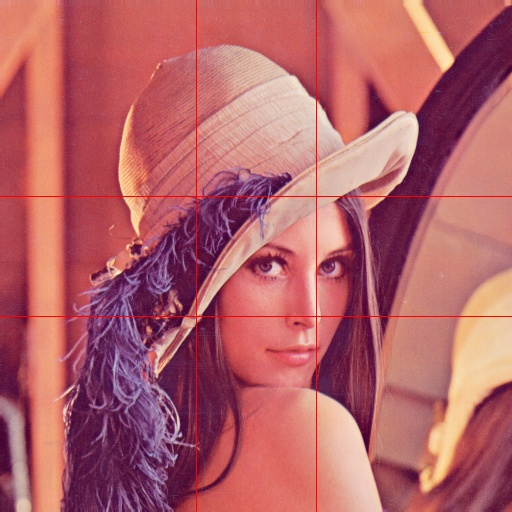
\includegraphics[scale=0.42,angle=0]{afsnit/vores_implementation/billeder/naiv_algoritme/Lenagolden}
	\end{center}
	\caption[]{Billedet som har indtegnet de fire gyldne snit}
	\label{lenasnit2}
\end{figure}

\begin{figure}[h]
	\begin{center}
		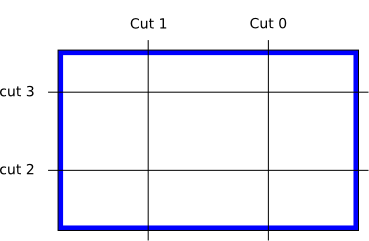
\includegraphics[scale=0.42,angle=0]{afsnit/vores_implementation/billeder/naiv_algoritme/Cut}
	\end{center}
	\caption[]{Billedets højde og bredde betegnes hvv. H og B. De 4 snit er navngivet.}
	\label{cut}
\end{figure}

De 4 snit tildeles hvert deres Id, "snit 0,1,2 og 3" så vi kan kende
forskel på de individuelde snit, Id'erne placering kan ses i figur
\ref{cut}. Vi vil i resten af rapporten kalde snittene efter deres Id.
Hvis vi gerne vil finde snittet som ligger i miden kommer der kun 2
snit, med vær deres Id "snit 0 og 1" som kan ses i figur \ref{Cut2}

\begin{figure}[h]
	\begin{center}
		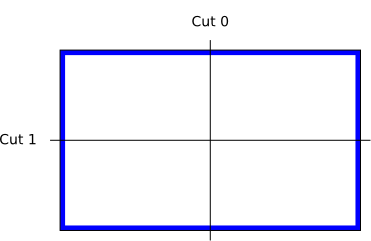
\includegraphics[scale=0.42,angle=0]{afsnit/vores_implementation/billeder/naiv_algoritme/2Cut}
	\end{center}
	\caption[]{Billedet skæres her kun af 2 snit}
	\label{2Cut}
\end{figure}

\subsection{Heltal i det gyldne snit}

I eksemplet med 4000 pixels ovenfor, approksimerer vi antal pixels ved
at afrunde resultatet $2472.13595 \approx 2472$, se udregning
\ref{afrundning}. Det betyder at vi mister 0.13595 pixels i præction,
hvilket svarer til en misvisning af punktet på 0.00339875 $\%$ i forholdt
til $B$ på billedet. Se udregning \ref{afrundning2}.

\begin{equation}
	4000 \cdot \varPhi = 4000(\sqrt{5}-1)/2 = 2472.13595 \approx 2472 \label{afrundning}
\end{equation}

\begin{equation}
	0.13595/4000 \cdot 100 = 0.00339875 \label{afrundning2}
\end{equation}

Det er en meget lille del af selve billedet og skulle ikke give nogle
misvisninger i forhold til udregningen. For at gøre det lidt mere
generelt, sætter vi trunkeringsfejlen til $0.5$, da det er den maksimale
afrundingsfacktor som kan forekomme. Hvis billedet har en størrelse på
500 pixels, hvilket er det mindste billedet vi har, giver dette en fejlmargin
på $0.1 \%$. Dette tal bliver adderet til fejlsatsen ovenfor, og giver
en samlet afvigelse på $2.1\%$.

\subsection{Snitratio}
End til vider har vi kun arbejder med det gyldne snit, men andre snit i
billedet kan godt optræde, derfor indføre vi en nu betegnelse
snitratio, som betegner en procents sats for hvor lang inde i billedet
snittet befinder sig. Det vil sige at hvis en snitration er på $0.2$. Et
billedet har $B$ på 4000 vil et snit befinde sig i pixel $4000*0.2 =
800$.

\subsection{Heltal ved udregning af Margin}
Når vi har 2 forskellige snitratioer, f.eks. $\varPhi$ og $\frac{2}{3}$,
som ligger meget tæt på hinanden, og vi gerne vil sammenligne hvilken
regioner der ligger i snitratioernens snit, er det vigtigt at margin for
vært af de 2 snitratioers snit ikke krydser hinanden. 

Hvis margin krydser. Vil det indebære, at den samme region bliver fundet
af begge snit. Dette vil give et skævt billedet af forskellen på de to.
Derfor må vi sørge for at marginerne ikke krydser. Hvis $x$ betegner
antal pixels i $B$ eller $H$, og vi vil se på, hvor mange pixels, der er
mellem snitratio $\frac{2}{3}$ og $\varPhi$, multiplicerer vi $x$ med de
to snitratioen for at finde deres placering. Derefter subtraheres vi et
af de snit som befinder sig tetest på hinanden i vær snitratio med
hinanden.


\begin{eqnarray}
	\frac{x2}{3} - \frac{x2}{\sqrt{5}+1} & = & x(\frac{2}{3} - \frac{2}{\sqrt{5} + 1}) \nonumber \\
	& = & x(0.666667-0.618034) \\ \nonumber
	& = & x(0.048633)
\end{eqnarray}

Vi har nu fundet antal pixel mellem de to snit. Vi vil gerne undgå at
de to marginer krydser hinanden, så vi dividere antal pixel mellem de to snit med to og afrunder værdien.

\begin{equation}
	\left\lfloor \frac{0.048633x}{2}\right\rfloor = \left\lfloor0.024316x \right\rfloor
	\label{marginstoerlse}
\end{equation}

Den minimale procentvise størrelse, margin må have, når vi
sammenligner det gyldne snit og $\frac{2}{3}$, er altså $2.4316$ Det
betyder også, at vi ikke må sammenligne snit som ligger særlig meget
tætter på hinanden, da $2.1\%$ er den minimale procent margin som vi må
have. For at vise, hvor stor marginen egentlige kan være, bruger vi formel \ref{marginstoerlse} på to billeder, et, som svarer til vores mindste billede, på
500 pixels, og et, som svarer til vores største billede, på 4000 pixels. Ved
500 pixels bliver resultatet.

\begin{definition}
	Margins størrelse i et snit, må ikke overstige $2.4316 \%$, af det respektive maleri $B$ eller $H$.
	\label{margin_max}
\end{definition}

\begin{definition}
	Margins størrelse i et snit, må ikke kommer under $2.1 \%$, af det respektice maleri $B$ eller $H$.
	\label{margin_min}
\end{definition}

\note{Er det denne måde det skal stilles op?}
\begin{equation}
	 \lfloor 500(0.024316)\rfloor = 12
\end{equation}

Det er en fin margin, da vores fejl på udregningerne ligger på 2.1 \%,
som svarer til $\lceil 500*0.021 \rceil = 11$ pixels. Der er 1 pixel fra vores
margin.

Ved 4000 pixels giver det.

\begin{equation}
	 \left\lfloor 4000(0.024316)\right\rfloor = 97
\end{equation}

Som også er god nok, da $4000*0.021 = 84$ pixels.
% vim: set tw=72 spell spelllang=da:
